%==================================================================
% BAB 3 — METODE PENELITIAN
%==================================================================

\chapter{METODE PENELITIAN}

\section{Jenis dan Pendekatan Penelitian}
Penelitian ini merupakan penelitian kuantitatif deskriptif. Pendekatan ini
dipilih karena tujuan penelitian adalah menggambarkan kondisi kualitas layanan
yang dirasakan pengguna dan menentukan prioritas perbaikannya, bukan menguji
hubungan sebab akibat antarvariabel.

\section{Tahapan Penelitian}
Penelitian dilaksanakan melalui tahapan yang ditunjukkan pada
\cref{fig:tahapan}. Tahapan disusun agar setiap keluaran menjadi masukan bagi
tahapan berikutnya.

\begin{figure}[H]
    \centering
    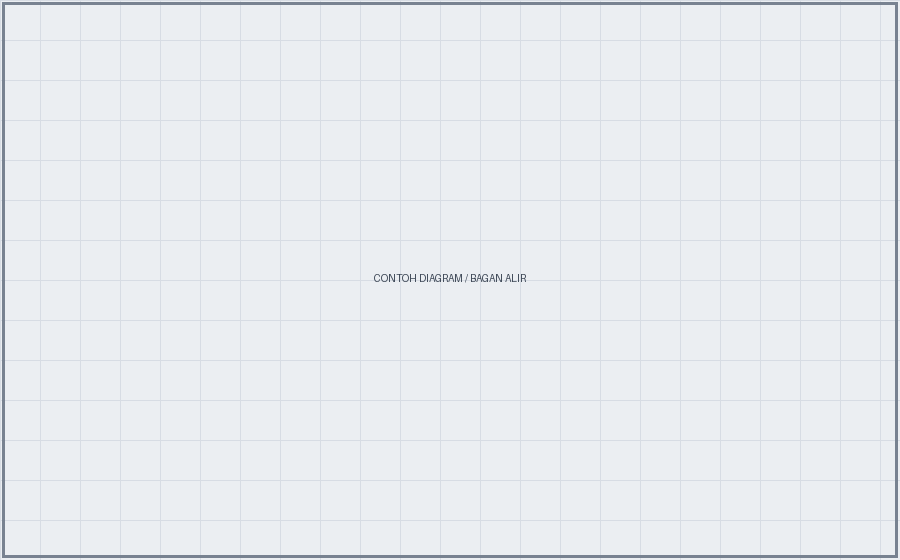
\includegraphics[width=0.75\linewidth]{contoh-diagram}
    \caption{Tahapan penelitian}
    \label{fig:tahapan}
\end{figure}

\begin{daftarnomor}
    \item \textbf{Studi pendahuluan.} Menelaah catatan layanan bantuan dan
          melakukan wawancara awal dengan pengelola sistem untuk memastikan
          masalah yang diteliti benar-benar terjadi.
    \item \textbf{Studi literatur.} Menelaah penelitian terdahulu dan landasan
          teori, serta menetapkan instrumen dan teknik analisis.
    \item \textbf{Penyusunan instrumen.} Menyiapkan kuesioner WebQual 4.0
          beserta terjemahan dan uji keterbacaannya.
    \item \textbf{Pengumpulan data.} Menyebarkan kuesioner kepada responden
          sesuai kriteria yang ditetapkan.
    \item \textbf{Pengujian instrumen.} Menguji validitas dan reliabilitas
          instrumen pada data yang terkumpul.
    \item \textbf{Analisis data.} Melakukan analisis deskriptif, analisis
          kesenjangan, dan pemetaan kuadran IPA.
    \item \textbf{Penarikan kesimpulan.} Menyusun kesimpulan yang menjawab
          setiap rumusan masalah.
\end{daftarnomor}

\section{Populasi dan Sampel}
Populasi penelitian adalah mahasiswa aktif yang telah menggunakan SIA minimal
dua semester, berjumlah 2.450 orang. Penentuan ukuran sampel menggunakan rumus
Slovin pada taraf kesalahan 10\% sebagaimana \cref{eq:slovin}.

\begin{equation}
    \label{eq:slovin}
    n = \frac{N}{1 + N e^{2}}
\end{equation}

\noindent dengan $n$ adalah ukuran sampel, $N$ adalah ukuran populasi, dan $e$
adalah taraf kesalahan. Berdasarkan perhitungan tersebut diperoleh ukuran
sampel minimum sebanyak 96 responden. Teknik pengambilan sampel yang digunakan
adalah \textit{purposive sampling} dengan kriteria inklusi berupa status
mahasiswa aktif dan pengalaman penggunaan minimal dua semester.

\section{Instrumen Penelitian}
Instrumen yang digunakan adalah WebQual 4.0 yang terdiri atas 22 butir pada tiga
dimensi. Setiap butir diukur pada dua skala Likert lima poin, yaitu tingkat
kepentingan dan tingkat kinerja. Instrumen digunakan tanpa penambahan maupun
pengurangan butir agar validitas aslinya tetap terjaga.

\section{Teknik Analisis Data}

\subsection{Pengujian Instrumen}
Validitas butir diuji menggunakan korelasi \textit{product moment}, dengan butir
dinyatakan valid apabila nilai $r_{hitung} > r_{tabel}$. Reliabilitas diuji
menggunakan koefisien \textit{Cronbach's alpha} sebagaimana \cref{eq:alpha},
dengan instrumen dinyatakan reliabel apabila nilainya di atas 0,70.

\begin{equation}
    \label{eq:alpha}
    \alpha = \frac{k}{k-1}\left(1 - \frac{\sum_{i=1}^{k} s_{i}^{2}}{s_{t}^{2}}\right)
\end{equation}

\noindent dengan $k$ adalah jumlah butir, $s_{i}^{2}$ adalah varians butir
ke-$i$, dan $s_{t}^{2}$ adalah varians skor total.

\subsection{Analisis Deskriptif}
Analisis deskriptif digunakan untuk menggambarkan tingkat kinerja setiap butir
dan setiap dimensi melalui nilai rata-rata dan simpangan baku.

\subsection{Analisis Kesenjangan}
Kesenjangan dihitung sebagai selisih antara rata-rata tingkat kinerja dan
rata-rata tingkat kepentingan pada setiap butir. Nilai negatif menunjukkan
kinerja yang belum memenuhi harapan pengguna.

\subsection{Importance-Performance Analysis}
Setiap butir dipetakan ke dalam diagram kartesius dengan sumbu mendatar berupa
tingkat kinerja dan sumbu tegak berupa tingkat kepentingan. Perpotongan sumbu
ditetapkan pada rata-rata keseluruhan, sehingga terbentuk empat kuadran:
prioritas utama, pertahankan prestasi, prioritas rendah, dan berlebihan.

\section{Matriks Keterkaitan Penelitian}

% MATRIKS INI ADALAH PENGAMAN PALING PENTING DALAM SELURUH NASKAH.
% Ia mencegah dua cacat yang paling sering terjadi:
%   (1) Bab 4 memuat pekerjaan yang tidak pernah ditanyakan di Bab 1;
%   (2) Bab 5 menjawab pertanyaan yang tidak pernah diajukan.
% Isi kolom terakhir HARUS menunjuk subbab yang benar-benar ada di Bab 4.

Keterkaitan antara rumusan masalah, tujuan, data, teknik analisis, dan penyajian
hasil disajikan pada \cref{tab:keterkaitan}. Matriks ini memastikan setiap
rumusan masalah benar-benar dijawab dan setiap hasil yang disajikan memang
ditanyakan.

\begin{table}[H]
    \centering
    \caption{Matriks keterkaitan penelitian}
    \label{tab:keterkaitan}
    \footnotesize
    \setlength{\tabcolsep}{4pt}
    \begin{tabular}{|c|p{2.9cm}|p{2.4cm}|p{3.3cm}|p{2.4cm}|}
        \hline
        \textbf{\labelrq} & \textbf{Tujuan} & \textbf{Data} &
        \textbf{Teknik analisis} & \textbf{Disajikan pada} \\ \hline

        \cref{rq:kualitas} & Mengukur tingkat kualitas layanan pada tiga dimensi &
        Skor kinerja 22 butir & Statistik deskriptif &
        Subbab \ref{sec:hasil-rq1} \\ \hline

        \cref{rq:kesenjangan} & Menganalisis kesenjangan kepentingan dan kinerja &
        Skor kepentingan dan kinerja & Analisis kesenjangan &
        Subbab \ref{sec:hasil-rq2} \\ \hline

        \cref{rq:prioritas} & Menentukan prioritas perbaikan &
        Hasil \cref{rq:kualitas,rq:kesenjangan} & \textit{Importance-\newline Performance Analysis} &
        Subbab \ref{sec:hasil-rq3} \\ \hline
    \end{tabular}
\end{table}

\section{Penggunaan Kecerdasan Buatan dalam Penelitian}
\label{sec:ai-penelitian}

Sesuai dengan prinsip transparansi dan integritas akademik, bagian ini
menjelaskan pemanfaatan teknologi kecerdasan buatan (\textit{Artificial
Intelligence}, AI) generatif dalam proses penelitian. Penggunaan AI dilakukan
secara terbatas, di bawah pengawasan penuh penulis, dan tidak menggantikan
penalaran, keahlian, maupun tanggung jawab penulis atas seluruh keputusan
penelitian.

\noindent\textbf{Catatan pemakaian templat:} isi subbab ini hanya bila AI benar-benar
digunakan pada proses \emph{penelitian} (mis. analisis data, penyusunan atau
pemeriksaan kode, perancangan struktur basis data). Bila AI hanya digunakan untuk
proses \emph{penulisan}, cukup gunakan halaman ``Pernyataan Penggunaan Kecerdasan
Buatan'' sebelum Daftar Pustaka. Bila AI tidak digunakan sama sekali, hapus subbab
ini beserta \texttt{\textbackslash include\{xx-deklarasi-ai\}} pada
\texttt{laporan.tex}.

Dalam penelitian ini, AI generatif (\belumdiisi{sebutkan nama dan versi alat,
mis. ChatGPT/GPT-4, Claude}) dimanfaatkan pada tahapan berikut:

\begin{daftarnomor}
    \item \textbf{Bantuan analisis atau pengolahan data.} \belumdiisi{jelaskan
          penggunaannya; seluruh perhitungan dan penafsiran diperiksa sendiri oleh
          penulis.}
    \item \textbf{Bantuan penyusunan atau pemeriksaan kode.} \belumdiisi{jelaskan
          penggunaannya; seluruh kode diverifikasi dan diuji sendiri oleh penulis.}
    \item \textbf{Bantuan perancangan struktur.} \belumdiisi{jelaskan
          penggunaannya; hasilnya divalidasi kesesuaiannya oleh penulis.}
\end{daftarnomor}

AI \textbf{tidak} digunakan untuk mengarang data, membuat hasil pengujian fiktif,
maupun menghasilkan sumber rujukan tanpa verifikasi. Seluruh keluaran AI telah
penulis periksa, sunting, dan validasi, sehingga penulis bertanggung jawab penuh
atas keakuratan dan integritas seluruh isi penelitian. Penggunaan AI untuk sekadar
pemeriksaan tata bahasa dan ejaan tidak termasuk yang dinyatakan di sini.
